% document formatting
\documentclass[10pt]{article}
\usepackage[utf8]{inputenc}
\usepackage[left=1in,right=1in,top=1in,bottom=1in]{geometry}
\usepackage[T1]{fontenc}
\usepackage{xcolor}

% math symbols, etc.
\usepackage{amsmath, amsfonts, amssymb, amsthm}

% lists
\usepackage{enumerate}

% images
\usepackage{graphicx} % for images
\usepackage{tikz}

% code blocks
\usepackage{minted, listings} 

% verbatim greek
\usepackage{alphabeta}

\newcommand{\dd}{\text{d}}

\graphicspath{{./assets/images/Week 5}}

\title{02-712 Week 5 \\ \large{Biological Modeling and Simulation}}
 
\author{Aidan Jan}

\date{\today}

\begin{document}
\maketitle

\section*{Deterministic Systems - Linear Model with Multiple Variables}
Depending on the type of problem, if it is possible to ignore probabilities, you should always try to do so
\begin{itemize}
	\item That is, abstract out the randomness of the biological system.
\end{itemize}

\subsection*{Example 1}
Condsider a bacterial growth system.  ($r$ is the rate.)
\begin{align*}
    \frac{\dd m}{\dd t} &= r \cdot m
\end{align*}
In this case, the solution is $m(t) = m(0) \cdot e^{rt}$.  If you can predict how the system starts, then you can predict how the system ends.  If $r > 0$, then the number of bacteria increase.  If $r < 0$, then the number of bacteria decrease.  Etc.\\\\
Suppose we want to find when the system is at equilibrium.  The system \textit{is} at equilibrium if $r = 0$, but we can't just change the $r$ since that is defined by how fast the bacteria divide.  Instead now, our only choice is to make $m(t) = 0$.\\\\
In general, for most systems we cannot just solve the differential equation, and we must instead make an estimate.

\subsubsection*{Phase Diagrams}
We can use phase diagrams to determine whether a equilibrium is stable.  A phase diagram (for now in 1D) is a number line, in which vectors are drawn in the direction of the derivative.  
\begin{itemize}
	\item In our example, if $r < 0$, then following the derivative formula, the number of bacteria would tend to zero.  (There are no negative bacteria!)  Therefore, equilibrium is stable.
	\item If $r > 0$, then following the derivative formula, the number of bacteria will explode and not stop at any number.  Therefore the equilibrium is not stable.
\end{itemize}
In general, an equilibrium is stable if when you keep applying the rule of change, the end result tends to some number.  An equilibrium is unstable if end result tends to an infinity.

\subsection*{Example 2}
Now, consider the system:
\begin{align*}
    \frac{\dd m_1}{\dd t} &= r_1 m_1(t)\\
    \frac{\dd m_2}{\dd t} &= r_2 m_2(t)
\end{align*}
This system has two variables (we are now on a 2D plane instead of a number line).
\begin{itemize}
    \item We can solve this system too.  (Since the two equations are independent from each other, it is same as the first system twice.)
    \begin{align*}
        m_1(t) &= m_1(0) e^{r_1 t}\\
        m_2(t) &= m_2(0) e^{r_2 t}
    \end{align*}
	\item By looking at this system, we know that the equilibrium is at $(0, 0)$.
	\item Also, since the two equations are independent, some things can be inferred about the biological system, such as, the two bacteria must not be competing for resources, space, etc.
	\item The phase diagram for this system is now a vector field on a 2D plane.
\end{itemize}
This problem is modeled with an \textbf{affine} model.  Essentially, describing the model using vectors and matrices.  We can rewrite this system as
\[\frac{\dd \vec{m}}{\dd t} = \begin{bmatrix} \frac{\dd m_1}{\dd t} \\ \frac{\dd m_2}{\dd t}\end{bmatrix} = M \begin{bmatrix} m_1 \\ m_2 \end{bmatrix}, \text{ where } M = \begin{bmatrix} r_1 & 0 \\ 0 & r_2 \end{bmatrix}\]
Therefore,
\[\frac{\dd \vec{m}}{\dd t} = M \cdot \vec{m} + \vec{C}\]

\subsection*{Example 3}
Consider now, the two populations of bacteria depend on each others' rates.
\begin{align*}
    \frac{\dd m_1}{\dd t} &= a m_1(t) + b m_2(t) \\
    \frac{\dd m_2}{\dd t} &= c m_1(t) + d m_2(t)
\end{align*}
Therefore, 
\[\frac{\dd \vec{m}}{\dd t} = M \vec{m}, \text{ where } M = \begin{bmatrix} a & b \\ c & d \end{bmatrix}\]
This model has only one equilibrium, provided that $\det(M) \neq 0$.
\begin{itemize}
	\item If $\det(M) = 0$, then there are an infinite number of solutions.  (Non-zero determinant means the matrix is invertible.)
\end{itemize}

\subsection*{Example 4}
Metastasis is a process in which cancer cells spread through the body.  Sometimes cancer cells move via the bloodstream and become lodged into capillaries, in which they start new tumors.  We will construct a model for the dynamics of the number of cancer cells lodged in the capillaries of an organ, $C$, and the number of cancer cells that have invaded the organ $I$.  Suppose that cells are lost from the capillaries by dislodgement or death at a per capita rate $\delta_1$ and that they invade the organ $I$ from the capillaries by a per capita rate $\beta$.  Once cells are in the organ $I$, they die at a rate of $\delta_2$, and the cancer cells in $I$ replicate at a per capita rate $\rho$.  All of the parameters are assumed positive.\\\\
First, we can summarize the information:
\begin{itemize}
	\item Parameters: $\delta_1, \delta_2, \beta, \rho$
	\item Variables: $C(t), I(t)$.  (Number of cancer cells in capillaries and organs, respectively)
	\item Assumptions: All parameters are positive.  No randomness.  Things not mentioned here don't matter.
\end{itemize}
Next, we can write the rules of change:
\begin{align*}
    \frac{\dd C}{\dd t} &= - C(t) \cdot (\delta_1 + \beta)\\
    \frac{\dd I}{\dd t} &= I(t) \cdot (\rho - \delta_2) + C(t) \cdot \beta
\end{align*}
Now, we can convert the system of differential equations into the affine form:
\[M = \begin{bmatrix} - \beta - \delta_1 & 0 \\ \beta & -\delta_2 + \rho \end{bmatrix}\]

\section*{Constrained Optimization}
Consider the following chemical reactions:
\begin{align*}
    A + 2B &\rightarrow C\\
    B + 2C &\rightarrow D
\end{align*}
and suppose we are adding 2 mol/sec of $A$ and 3 mol/sec of $B$.\\\\
This is another computational problem that we may come across, called the \textbf{flux balance analysis}.  We want to know how fast $D$ is produced.\\\\
To start, we can view this as a graph.

\begin{center}
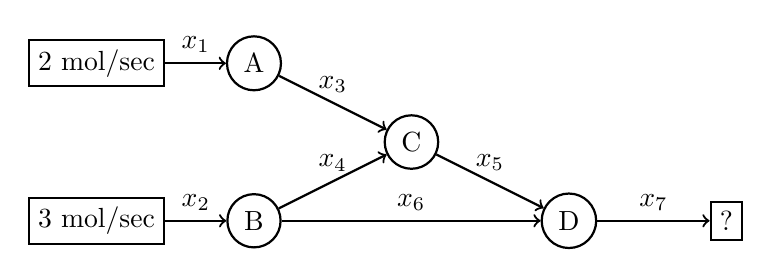
\begin{tikzpicture}
    \node[draw, thick] at (-2, 2) (sourceA) {2 mol/sec};
    \node[draw, thick] at (-2, 0) (sourceB) {3 mol/sec};
    \node[draw, thick, circle] at (0, 2) (A) {A};
    \node[draw, thick, circle] at (0, 0) (B) {B};
    \node[draw, thick, circle] at (2, 1) (C) {C};
    \node[draw, thick, circle] at (4, 0) (D) {D};
    \node[draw, thick] at (6, 0) (output) {?};

    \draw[->, thick] (sourceA) edge node[above] {$x_1$} (A);
    \draw[->, thick] (sourceB) edge node[above] {$x_2$} (B);
    \draw[->, thick] (A) edge node[above] {$x_3$} (C);
    \draw[->, thick] (B) edge node[above] {$x_4$} (C);
    \draw[->, thick] (C) edge node[above] {$x_5$} (D);
    \draw[->, thick] (B) edge node[above] {$x_6$} (D);
    \draw[->, thick] (D) edge node[above] {$x_7$} (output);
\end{tikzpicture}
\end{center}
From this graph, we can infer a few things about the system:
\begin{align*}
    x_1 &\leq 2\\
    x_2 &\leq 3\\
    x_3 &\leq x_1 \\
    x_4 + x_6 &\leq x_2 \\
    x_5 &\leq x_3 \\
    x_5 &\leq \frac{1}{2} x_4 \\
    x_7 &\leq x_6\\
    x_7 &\leq \frac{1}{2} x_5
\end{align*}
And our objective is for $x_1, x_2, x_3, x_4, x_5, x_6, x_7 \geq 0$.\\\\
\textbf{To solve this}, we can use a linear program (LP).
\begin{enumerate}
	\item Set of variables $\vec{x} = \{x_1, \dots, x_n\}$
	\item Set of linear constraints
	\[\sum_{i = 1}^n a_i, x_i \leq b_i, \quad A\vec{x} \leq \vec{b}\]
    \item Linear objective:
    \[\min_{} \sum_{i = 1}^n Cx_i = \min \vec{C}^T \vec{x}\]
\end{enumerate}
If we want to minimize $x_1 + x_2$, then we can write the system:
\begin{align*}
    x_1 &\geq 0\\           
    x_2 &\geq 0 \\          
    x_1 + 2x_2 &\leq 8\\
    x_1 - x_2 &\leq 2
\end{align*}
From this, we can derive:
\begin{align*}
    \vec{x} &= (x_1, x_2)\\
    \vec{c} &= (1, 1)\\
    A &= \begin{bmatrix} 1 & 2 \\ 1 & -1 \\ -1 & 0 \\ 0 & -1\end{bmatrix}\\
    \vec{b} &= \begin{bmatrix} 8 \\ 2 \\ 0 \\ 0 \end{bmatrix}
\end{align*}
If we graph these inequalities, then one section of the graph (where the two inequalities overlap) would be all the feasible solutions.  However, not all of them are optimal.
\begin{itemize}
    \item Optimizing two variables is done in a 2D cartesian plane, with lines separating the regions
    \item Three variables would be graphed in a 3D space, with planes separating the regions.
    \item Four variables use a 4D space, with hyperplanes as dividers.
\end{itemize}
\subsubsection*{Finding the Optimal}
We have multiple ways of finding the optimal solution, but one way is the \textbf{simplex method}.  The simplex theorem states that the optimal solution must be at one of the vertices of the feasible section.  (Vertices defined as the point where inequalities intersect, where they intersect the $x$ and $y$-axes, the origin, etc.)
\begin{itemize}
	\item Therefore, we can start at one of the vertices, test the values, then slide along an edge to another vertex, check the values again, etc. and gradient descent our way to the correct vertex.  Once we get there, there will be no way to improve, and it is the global minimum for the problem.
	\item In practical applications, this is easier said than done.  Typically we have way more than 2 variables, so much optimization is needed.
\end{itemize}

\subsection*{Standard Form}
The \textbf{standard form} of a continued optimization is the following:
\begin{itemize}
	\item We want to minimize $c_1 x_1 + c_2 x_2 + \dots + c_n x_n$.  We have matrix $A$ and the vector $\vec{x}$ (our inputs), and $\vec{b}$ (our outputs).
	\item We want the form $A\vec{x} = \vec{b}$.
	\item From here, we can implement the simplex method on the system.
\end{itemize}
To get a problem to standard form, we have four cases:
\begin{enumerate}
	\item If we have $\vec{a_i}^T \vec{x} \geq b$ (we don't want greater than sign), then we can rewrite it as $-\vec{a_1}^T \vec{x} \leq -b_j$
	\item If we have $\vec{a_i}^T \vec{x} \leq b_j$ (), we can rewrite it as $\vec{a_i}^T \vec{x} + \vec{x_i} = b_j$.  We can add a slack variable $\vec{x}$, where $\vec{x} \geq 0$
	\item If $x_i$ might be negative, then we write $x_i = (x_{i+} - x_{i-})$, where $x_{i+}, x_{i-} \geq 0$.  In other words, we write $x_i$ as a difference between two variables.
	\item Finally, if we have a maximization problem, e.g., $\max \vec{C}^T \vec{x}$, we rewrite it as $\min -\vec{C}^T \vec{x}$.
\end{enumerate}

\subsection*{Simplex Algorithm}
\begin{enumerate}
	\item Pick initial feasible point, and set $n - m$ variables to zero
	\item Rewrite in terms of zero variables, and solve for non-zero variables
	\item Find $x_i$ with negative coefficient in objective (or quit if none exists)
	\item Increase $x_i$ until some $x_i \rightarrow 0$.
	\item Return to Step 2.
\end{enumerate}

\subsection*{Example}
Suppose we have a linear program:
$\max x_1 + 3x_2 \text{ such that}$
\begin{align*}
    x_1 - x_2 &\geq -4\\
    x_1 + x_2 &\leq 10\\
    x_1 &\geq 0\\
    x_2 &\geq 0
\end{align*}
First, we need to rewrite so there are no greater thans.
\begin{align*}
    -x_1 + x_2 &\leq 4\\
    x_1 + x_2 &\leq 10\\
    x_1 &\geq 0\\
    x_2 &\geq 0
\end{align*}
Now, we need to get rid of the $-x_1$, so we need to substitute with one variable subtract another.
\begin{align*}
    x_1 + x_2 + x_3 &\leq 4\\
    x_1 + x_2 + x_4 &\leq 10\\
    x_1 &\geq 0\\
    x_2 &\geq 0\\ 
    x_3 &\geq 0\\
    x_4 &\geq 0
\end{align*}
Our final program is:
$\min -x_1 - 3x_2$ such that:
\begin{align*}
    x_1 + x_2 + x_3 &\leq 4\\
    x_1 + x_2 + x_4 &\leq 10\\
    x_1, x_2, x_3, x_4 &\geq 0
\end{align*}
Since we have two inequalities but four variables, we can set two to zero.  We will set $x_1$ and $x_2$ to zero, arbitrarily.
\begin{align*}
    x_3 &= x_1 - x_2 + 4\\
    x_4 &= -x_1 - x_2 + 10\\
    x_1 = x_2 &= 0
\end{align*}
Therefore, our variables have the solution $(0, 0, 4, 10)$.\\\\
From here, we can use the simplex method.  $(0, 0, 4, 10)$ is a solution, but not optimal.  Our objective function, $-x_1 - 3x_2$ is currently 0.
\begin{itemize}
	\item Let's choose to increase $x_2 \rightarrow 4$ and $x_3 \rightarrow 0$.  Now our objective is $-12$.
\end{itemize}
We can now rewrite our constraints in terms of $x_2$ instead:
\begin{align*}
    x_2 &= x_1 - x_3 + 4\\
    x_4 &= -x_2 - (x_1 - x_3 + 4) + 10 \\
    &\rightarrow -2x_1 + x_3 + 6
\end{align*}
And also rewrite our objective: $\min -4x_1 + 3x_3 - 12$.
\begin{itemize}
	\item Can we improve our solution?  Let's increase $x_1 \rightarrow 3$, and $x_4 \rightarrow 0$. 
\end{itemize}
Rewriting again, we get
\begin{align*}
    x_1 &= \frac{1}{2} x_3 - \frac{1}{2} x_4 + 3\\
    x_2 &= -\frac{1}{2} x_3 - \frac{1}{2} x_4 + 7
\end{align*}
And also our objective is $\min x_3 + 2x_4 - 24$.  Plugging in $x_3 = x_4 = 0$, we get a value of $-24$.  This is now optimal, since both our slack variables, $x_3$ and $x_4$ are now zero.
\begin{itemize}
	\item We can now solve for the values of $x_1$ and $x_2$ based on our rewritten equations and plugging in $0$, which gives 
	\begin{align*}
        x_1 &= 3 \\
        x_2 &= 7
    \end{align*}
    \item These are the optimal solutions in the original coordinate space.
\end{itemize}

\subsection*{Affine Method (Interior Point Method)}
This is a variant of the simplex method that allows choices of points in the feasible area rather than just on the edges of the feasible area.
\begin{enumerate}
	\item Start with a feasible $\vec{x_0}$
	\item Transform coordinates such that it moves $\vec{x_1}$ away from the boundary.\\
	      $x_i \geq 0$, $x_i \rightarrow x_i'$.  Let $X = \begin{bmatrix} x_1 & 0 \\ 0 & x_2\end{bmatrix}$.  Let $\vec{x_1}' = X^{-1} \vec{x}$.
	\item Find $-\nabla g = -\vec{C}$
	\item Project $-\vec{c}$ into the null space of $A$.
    \begin{align*}
        A\vec{v_1} &= \vec{0}\\
        A\vec{v_2} &= \vec{0}
    \end{align*}
\end{enumerate}
Steps 3 and 4 effectively move the point back to the edge, and convert the coordinate system back to the original.  Doing this over and over again is basically a gradient descent algorithm, and in high dimensions it beats searching through all the combinations of variables.

\section*{Convex Programs}
In a convex program, the constraints are defined by a convex set $S$.
\begin{itemize}
	\item $x, y \in S$, $\alpha x + (1 - \alpha)y \in S$, $\alpha \in [0, 1]$.
	\item Basically, if you pick any two points $x$ and $y$ in $S$, and you draw a straight line connecting them, all the points of the line are inside the set too.
	\item A circle is a convex set.  (You can pick any two points in it and draw a line, and you will still be inside.)
	\item A crescent is not a convex set.  (If you pick points at the 'tips' of the crescent and draw a line, the line will leave the set.)
\end{itemize}





\end{document}